\documentclass[12pt, psamsfonts]{amsart}

%-------Packages---------
\usepackage{amssymb,amsfonts}
\usepackage{mathtools}
\usepackage{semantic}
\usepackage{fullpage}
\usepackage{tikz-cd}
\usepackage{todonotes}
\usepackage{physics}
\usepackage[all,arc]{xy}
\usepackage{enumerate}
\usepackage{enumitem}
\usepackage{mathrsfs}
\usepackage{theoremref}
\usepackage{graphicx}
\usepackage[bookmarks]{hyperref}

%--------Theorem Environments--------
%theoremstyle{plain} --- default
\newtheorem{thm}{Theorem}[section]
\newtheorem{cor}[thm]{Corollary}
\newtheorem{prop}[thm]{Proposition}
\newtheorem{lem}[thm]{Lemma}
\newtheorem{conj}[thm]{Conjecture}
\newtheorem{quest}[thm]{Question}

\theoremstyle{definition}
\newtheorem{defn}[thm]{Definition}
\newtheorem{defns}[thm]{Definitions}
\newtheorem{con}[thm]{Construction}
\newtheorem{exmp}[thm]{Example}
\newtheorem{exmps}[thm]{Examples}
\newtheorem{notn}[thm]{Notation}
\newtheorem{notns}[thm]{Notations}
\newtheorem{addm}[thm]{Addendum}
\newtheorem*{exer}{Exercise}

\theoremstyle{remark}
\newtheorem{rem}[thm]{Remark}
\newtheorem{rems}[thm]{Remarks}
\newtheorem{warn}[thm]{Warning}
\newtheorem{sch}[thm]{Scholium}

\DeclareMathOperator{\Hom}{Hom}
\DeclareMathOperator{\Id}{Id}
\DeclareMathOperator{\End}{End}
\DeclareMathOperator{\ord}{ord}
\DeclareMathOperator{\Aut}{Aut}
\DeclareMathOperator{\Gal}{Gal}

\makeatletter
\let\c@equation\c@thm
\makeatother
\numberwithin{equation}{section}

\bibliographystyle{plain}

\begin{document}

\title{Math 611 Final}
\author{Hidenori Shinohara}
\maketitle

\begin{exer}{(Problem 2)}
 \begin{figure}
   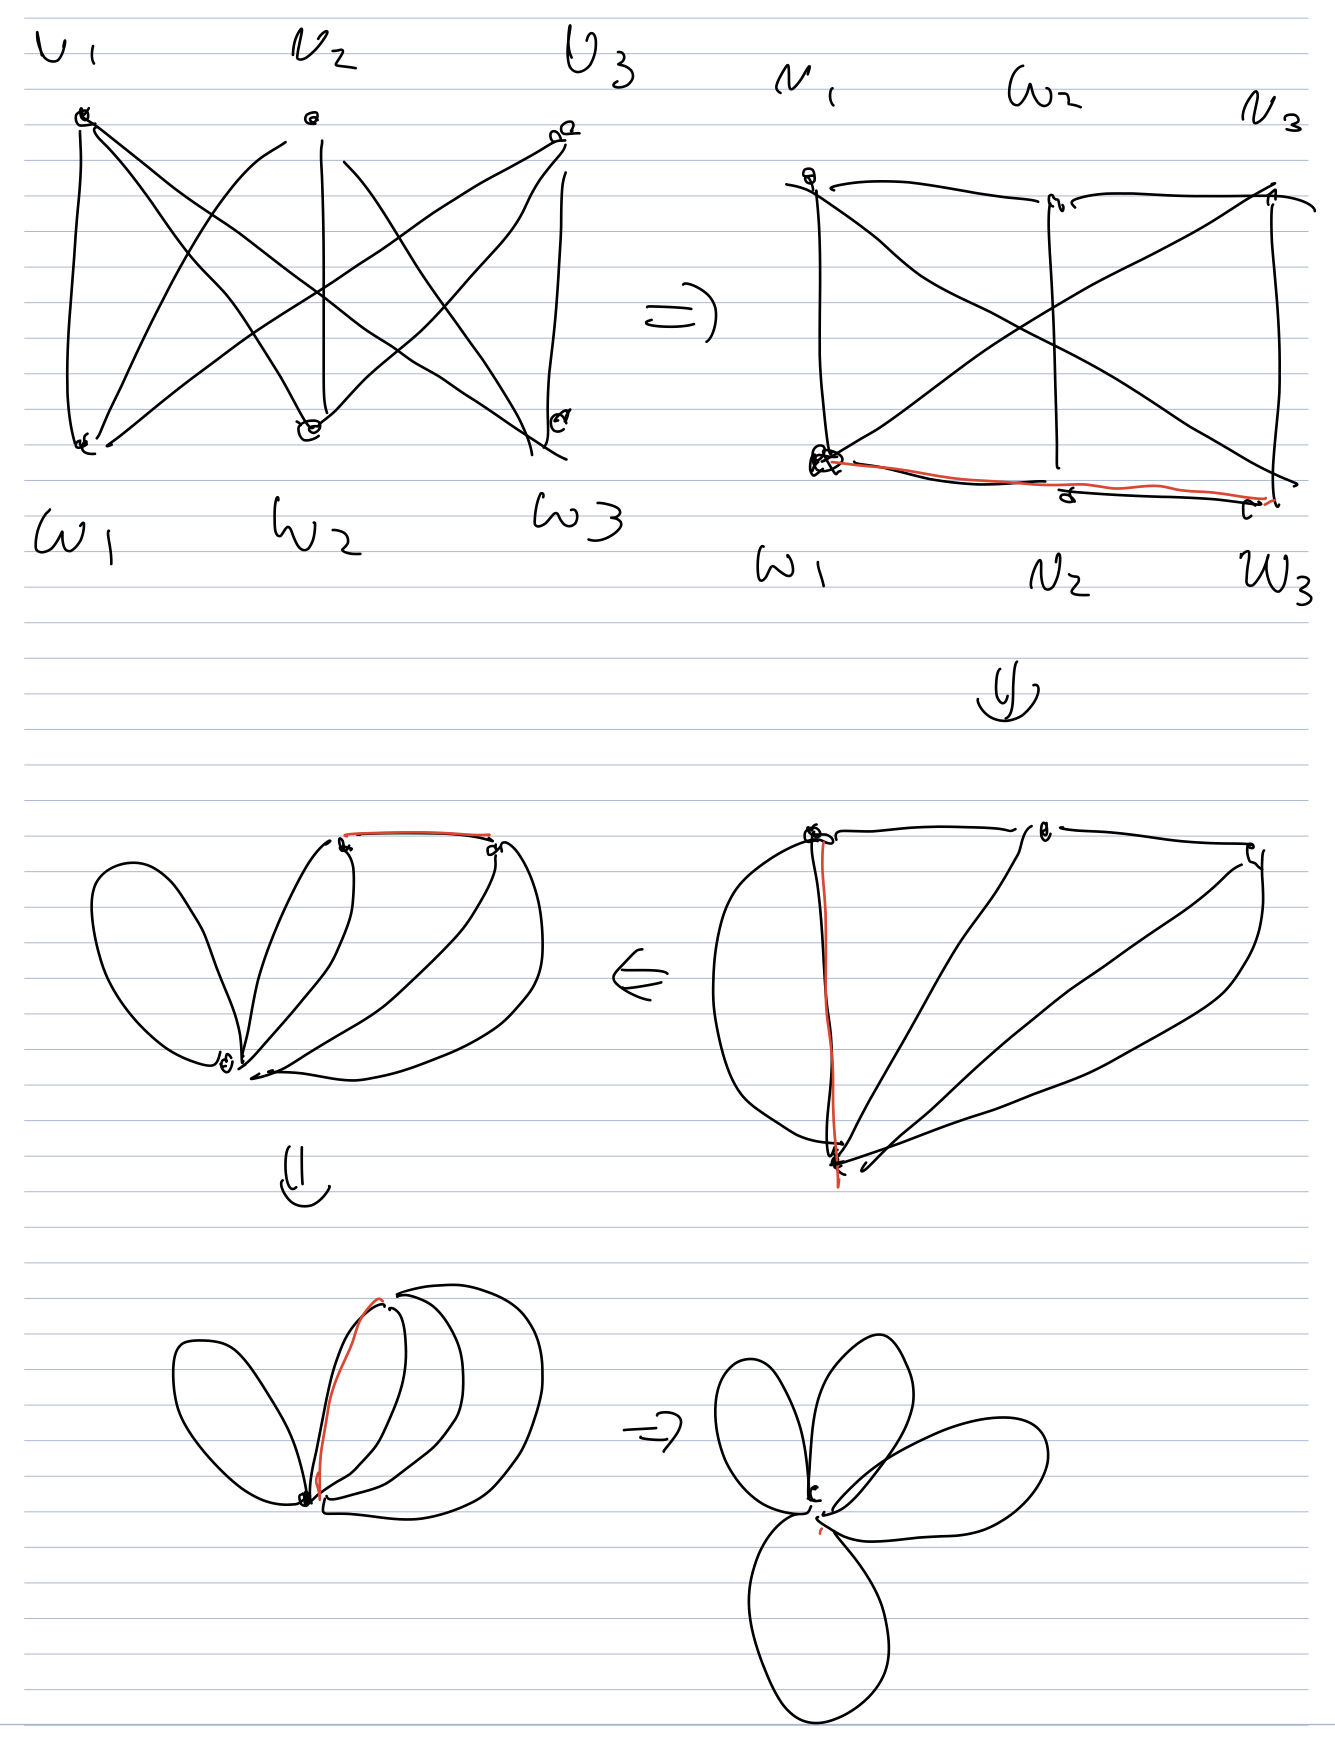
\includegraphics[width=.5\linewidth]{k33.jpeg}
   \caption{$K_{3, 3}$}
   \label{fig:k33}
 \end{figure}
 Figure \ref{fig:k33} shows how $K_{3, 3}$ is homotopy equivalent to $S_1 \vee S_1 \vee S_1 \vee S_1$.
 Thus the Van Kampen theorem implies that the fundamental group is the free group generated by 4 elements $\ev{ a, b, c, d }$ where each generator corresponds to each $S_1$.
\end{exer}

\begin{exer}{(Problem 5(a))}
  Let $X = S^1 \times S^2$ and $Y = S^1 \vee S^2 \vee S^3$.
  \begin{align*}
    \pi_1(S^1 \times S^2)
      &= \pi_1(S^1) \times \pi_1(S^2) & \text{(Proposition 1.12)} \\
      &= \mathbb{Z} \times 0 \\
      &= \mathbb{Z}. \\
    \pi_1(S^1 \vee S^2 \vee S^3)
      &= \pi_1(S^1) * \pi_1(S^2) * \pi_1(S^3) & \text{(Van Kampen)} \\
      &= \mathbb{Z} * 0 * 0 \\
      &= \mathbb{Z}.
  \end{align*}

  $X$ and $Y$ are both path connected, so $H_0(X) = H_0(Y) = \mathbb{Z}$.

  We will consider two subspaces of $X$ the union of whose interiors equals $X$.
  Identify each point of $X = S^1 \times S^2$ by a pair of coordinates $(\theta, (x, y, z))$ where $\theta$ is the angle in $S^1$ and $(x, y, z)$ satisfies $x^2 + y^2 + z^2 = 1$.
  Let $A = \{ (\theta, (x, y, z)) \mid -\epsilon \leq \theta \leq \pi + \epsilon \}, B = \{ (\theta, (x, y, z)) \mid \pi - \epsilon \leq \theta \leq 2\pi + \epsilon \}$ where $\epsilon > 0$ is a small number.
  Then each $A$ and $B$ deformation retracts to a space homeomorphic to $S^2$.
  $A \cap B$ consists of two path components, each of which deformation retracts to a space homeomorphic to $S^2$.
  The homology groups of $A \cap B$ are relatively easy to calculate because $H_n(A \cap B) = H_n(S^2 \coprod S^2) = H_n(S^2) \oplus H_n(S^2)$ by Proposition 2.6 for any $n$.
  Moreover, it is clear that $\int(A) \cup \int(B) = X$.
  We will consider the Mayer-Vietoris sequence formed by $A, B \subset X$.

  First, we will consider the sequence $H_n(A) \oplus H_n(B) \rightarrow H_n(X) \rightarrow H_{n - 1}(A \cap B)$ for each $n \geq 4$.
  $H_n(A) = H_n(B) = H_{n - 1}(A \cap B) = 0$ for $n \geq 4$
  By the exactness, $H_n(X) = 0$ for all $n \geq 4$.
  Next, we will consider the following sequence:

  \begin{align*}
    &\tilde{H}_3(A \cap B) \rightarrow \tilde{H}_3(A) \oplus \tilde{H}_3(B) \rightarrow \tilde{H}_3(X) \xrightarrow{\alpha} \\
    &\tilde{H}_2(A \cap B) \xrightarrow{\beta} \tilde{H}_2(A) \oplus \tilde{H}_2(B) \xrightarrow{\gamma} \tilde{H}_2(X) \rightarrow \\
    &\tilde{H}_1(A \cap B) \rightarrow \tilde{H}_1(A) \oplus \tilde{H}_1(B) \rightarrow \tilde{H}_1(X) \rightarrow \\
    &\tilde{H}_0(A \cap B) \rightarrow \tilde{H}_0(A) \oplus \tilde{H}_0(B).
  \end{align*}

  $\tilde{H}_3(A \cap B) = \tilde{H}_3(A) = \tilde{H}_3(B) = \tilde{H}_1(A \cap B) = \tilde{H}_1(A) = \tilde{H}_1 = \tilde{H}_0(A) = \tilde{H}_0(B) = 0$, and $\tilde{H}_0(A \cap B)$.
  By replacing the exact sequence with those values and splitting the sequence into two for readability, we obtain the following sequences:
  \begin{gather*}
    0 \rightarrow \tilde{H}_3(X) \xrightarrow{\alpha} \tilde{H}_2(A \cap B) \xrightarrow{\beta} \tilde{H}_2(A) \oplus \tilde{H}_2(B) \xrightarrow{\gamma} \tilde{H}_2(X) \rightarrow 0, \\
    0 \rightarrow \tilde{H}_1(X) \rightarrow \mathbb{Z} \rightarrow 0.
  \end{gather*}

  By the exactness, we can conclude that $\tilde{H}_1(X) \cong \mathbb{Z}$.
  We will examine the homomorphism $\beta$ to understand the sequence.
  $\tilde{H}_2(A \cap B) = \ev{[a], [b] \mid [[a], [b]]}$ where each $a, b$ lives in $A \cap B$ and $a$ lives in one of the path components of $A \cap B$ and $b$ lives in the other.
  Moreover, $[a] = [b]$ in $\tilde{H}_2(A)$ and $\tilde{H}_2(B)$.
  (Based on orientation, $[a] = -[b]$, but we can simply change the orientation of $[b]$ in that case.)
  Then $\beta(c_1[a] + c_2[b]) = ((c_1 + c_2)[a], (c_1 + c_2)[a])$.
  This gives us that $\Im(\alpha) = \ker(\beta) = \{ c[a] - c[b] \mid c \in \mathbb{Z} \} = \mathbb{Z}$.
  By the exactness, $\alpha$ is injective, so $\tilde{H}_3(X) = \mathbb{Z}$.
  Moreover, $\ker(\gamma) = \Im(\beta) = \{ (c[a], c[a]) \mid c \in \mathbb{Z} \}$.
  By the exactness, $\gamma$ is surjective, so $\tilde{H}_2(X) = (\tilde{H}_2(A) \oplus \tilde{H}_2(B)) / \Im(\beta) = \ev{[a]} \oplus \ev{[a]} / \ev{([a], [a])} = \mathbb{Z}$.
  Since reduced homology groups and homology groups are identical when $n \geq 2$, we have
  \begin{align*}
    H_n(X) &= \begin{cases}
      \mathbb{Z} & (n = 0, 1, 2, 3) \\
      0 & (n \geq 4).
    \end{cases}
  \end{align*}


  By Corollary 2.25, $\tilde{H}_n(S^1 \vee S^2 \vee S^3) = \tilde{H}_n(S^1) \otimes \tilde{H}_n(S^2) \otimes \tilde{H}_n(S^3)$.

  Therefore,
  \begin{align*}
    \tilde{H}_n(Y) = \begin{cases}
      \mathbb{Z} & (n = 1, 2, 3) \\
      0 & (n = 0, n \geq 4).
    \end{cases}
  \end{align*}

  For $n \geq 1$, $\tilde{H}_n(Y) = H_n(Y)$, so $H_0(Y) = H_1(Y) = H_2(Y) = H_3(Y) = \mathbb{Z}$ and $H_n(Y) = 0$ for all $n \geq 4$.
\end{exer}

\begin{exer}{(Problem 5(b))}
  We claim that the universal cover is $\mathbb{R} \times S^2$.
  $p(\theta, (x, y, z)) = ((\cos \theta, \sin \theta), (x, y, z))$ is a covering map.
  Moreover, $\pi_1(\mathbb{R} \times S^2) = \pi_1(\mathbb{R}) \times \pi_1(S^2) = 0 \times 0 = 0$, so $\mathbb{R} \times S^2$ is simply connected.
  Therefore, $\mathbb{R} \times S^2$ is indeed a universal cover of $X$.

  $\mathbb{R} \times S^2$ is homeomorphic to $(0, 1) \times S^2$.
  This space deformation retracts to $S^2$ because $(0, 1) \times S^2$ is homeomorphic to an open ball with its center removed.
  Thus their homology groups are $H_2(\tilde{X}) = H_0(\tilde{X}) = \mathbb{Z}$ and $H_n(\tilde{X}) = 0$ for all other $n$.
\end{exer}

\begin{exer}{(Problem 5(c))}
  The real line with $S^2 \vee S^3$ attached to each of its integral points.
  \todo[inline,caption={}]{
    Calculate its homology groups.
  }
\end{exer}

\end{document}


